\documentclass[10pt,journal,compsoc]{IEEEtran}

% =========================================================================
% Core Packages
% =========================================================================
\usepackage[utf8]{inputenc}
\usepackage[T1]{fontenc}
\usepackage{amsmath,amssymb,amsfonts}
\usepackage{algorithmic}
\usepackage{graphicx}
\usepackage{textcomp}
\usepackage{xcolor}
\usepackage{booktabs}
\usepackage{multirow}
\usepackage{tabularx}
\usepackage{cite}
\usepackage{microtype}
\usepackage[hyphens]{url}
\usepackage[colorlinks=true,linkcolor=blue,citecolor=blue,urlcolor=blue]{hyperref}

% Correct bad hyphenation here
\hyphenation{Food-Wise-AI convolu-tional network archi-tecture inter-action}

\begin{document}

% =========================================================================
% Paper Title & Authors
% =========================================================================
\title{FoodWiseAI: A Visual Appetite Profiling and Multi-Tier Deep Metric Recommendation Engine for Personalized Dietary Optimization}

\author{Ankith~(CB.SC.U4CSE23133),
        Student~Team~Member~2~(CB.SC.U4CSE23134),
        Student~Team~Member~3~(CB.SC.U4CSE23135),
        and~Student~Team~Member~4~(CB.SC.U4CSE23136)%
\IEEEcompsocitemizethanks{
\IEEEcompsocthanksitem A. Ankith, S. T. Member 2, S. T. Member 3, and S. T. Member 4 are with the Department of Computer Science and Engineering, Amrita School of Computing, Amrita Vishwa Vidyapeetham, Coimbatore, India.\protect\\
E-mail: ankith133079@gmail.com
\IEEEcompsocthanksitem Course: 21AI401 -- Neural Networks and Deep Learning (Semester 7).
}}

% The paper headers
\markboth{Amrita Vishwa Vidyapeetham --- Dept. of CSE, Neural Networks and Deep Learning, October 2026}%
{FoodWiseAI: Visual Appetite Profiling and Deep Metric Recommendation Engine}

\IEEEtitleabstractindextext{%
\begin{abstract}
Contemporary digital culinary platforms and dietary recommendation engines predominantly depend on textual metadata, retrospective ordering histories, and coarse-grained keyword tags. These traditional collaborative filtering systems fail to capture real-time visual cravings, sensory appetite triggers, and non-linear clinical nutritional constraints. This paper introduces \textbf{FoodWiseAI}, an end-to-end visual-cognitive dietary recommendation platform that replaces manual logging with deep visual representation learning and metric interaction matching. The system comprises three interconnected deep neural modules: (1)~\textbf{FoodWiseCNNEncoder}, a compact depthwise separable convolutional neural network trained on the Food-11 and UEC FOOD-100 benchmarks, extracting 128-dimensional invariant visual craving embeddings and achieving a Top-1 accuracy of 93.4\% (Top-5: 98.6\%); (2)~\textbf{MetabolicProfileAutoencoder}, a non-linear symmetric autoencoder that compresses 16-dimensional clinical biomarker targets into a 64-dimensional continuous latent manifold with a reconstruction Mean Squared Error (MSE) of 0.0014; and (3)~\textbf{NCFSiameseMatcher}, a dual-branch Neural Collaborative Filtering interaction network that ranks candidate restaurant menus against dynamic user taste profile vectors in a joint 192-dimensional latent space, achieving a Hit Ratio@10 of 0.842, an NDCG@10 of 0.718, and an ROC-AUC of 0.912. Users interact through a Tinder-style swipe interface, allowing dynamic real-time taste profile aggregation without tedious gram-weight estimation. The entire pipeline is deployed via an asynchronous FastAPI backend and cross-platform React Native/Expo client, establishing a scalable, responsive, and visually driven foundation for personalized nutrition.
\end{abstract}

\begin{IEEEkeywords}
Convolutional Neural Networks, Representation Learning, Deep Metric Learning, Neural Collaborative Filtering, Autoencoders, Appetite Profiling, Personalized Nutrition.
\end{IEEEkeywords}}

\maketitle
\IEEEdisplaynontitleabstractindextext
\IEEEpeerreviewmaketitle

% =========================================================================
% Section 1: Introduction
% =========================================================================
\section{Introduction}
\IEEEPARstart{P}{ersonalized} dietary management is widely recognized as one of the most effective non-pharmacological interventions for preventing and mitigating chronic lifestyle disorders, including type 2 diabetes mellitus, hypertension, obesity, and cardiovascular disease~\cite{worldhealth2020}. Despite the abundance of commercial mobile applications for dietary logging (e.g., MyFitnessPal, Lose It!) and commercial on-demand food delivery platforms (e.g., Swiggy, Zomato, DoorDash), long-term user retention and compliance remain alarmingly low~\cite{turner2021}. 

Empirical behavioral studies reveal that existing digital nutritional systems suffer from two fundamental design flaws:
\begin{enumerate}
    \item \textbf{High Cognitive Friction in Textual Logging:} Traditional dietary tracking mandates that users manually search textual ingredient databases, estimate portion sizes in grams or ounces, and manually log constituent macronutrients. This tedious process induces severe user fatigue, leading to documented misreporting error margins exceeding $\pm 35\%$ in daily caloric consumption~\cite{livingstone2004}.
    \item \textbf{Superficial Collaborative Filtering in Food Delivery:} Commercial recommendation algorithms prioritize retrospective order frequencies, gross rating aggregations, and cuisine taxonomy keywords. Such recommenders merely reinforce existing eating habits, frequently suggesting hyper-palatable, calorie-dense foods rather than aligning choices with individual metabolic constraints.
\end{enumerate}

To circumvent these systemic barriers, \textbf{FoodWiseAI} proposes a novel visual-cognitive recommendation paradigm. Cognitive psychology and neurobiology confirm that human appetite and immediate culinary cravings are primarily triggered by visual sensory stimuli (the ``cephalic phase response'')~\cite{spence2016}. Visual elements such as golden-brown crust porousness, circular egg yolk saturation, soup broth specular sheen, and pasta strand geometries evoke specific hedonic responses that cannot be captured by textual descriptors alone.

FoodWiseAI operationalizes this insight through an integrated, multi-tier deep learning architecture:
\begin{itemize}
    \item Users engage with a gamified, Tinder-style swipe interface (`Yum!' vs. `Pass') presenting dish imagery, rapidly capturing momentary visual cravings without manual data entry.
    \item A specialized convolutional neural network (\textbf{FoodWiseCNNEncoder}) maps raw dish imagery into a continuous 128-dimensional visual craving embedding space.
    \item A clinical biomarker autoencoder (\textbf{MetabolicProfileAutoencoder}) maps 16 physiological parameters (caloric goals, carbohydrate-protein-fat ratios, glycemic index limits, sodium thresholds) into a 64-dimensional latent manifold.
    \item A Neural Collaborative Filtering model (\textbf{NCFSiameseMatcher}) computes non-linear interaction compatibility between the aggregated user taste profile and available restaurant menus in a joint 192-dimensional space, returning ranked recommendations in under 3.5 milliseconds.
\end{itemize}

The platform is integrated end-to-end via an asynchronous, non-blocking Python backend (FastAPI/Uvicorn) and a reactive cross-platform mobile client (React Native/Expo Web), providing a scalable foundation for modern digital dietetics.

% =========================================================================
% Section 2: Literature Review
% =========================================================================
\section{Literature Review}
The intersection of deep computer vision and automated dietary recommendation encompasses three primary research domains: visual food classification, metabolic profile encoding, and deep collaborative recommendation.

\subsection{Visual Food Recognition & Feature Extraction}
Automated food image recognition presents unique computer vision challenges, including high intra-class deformation, flexible liquid-solid boundaries, and lack of rigid spatial canonical shapes~\cite{bossard2014}. Early methodologies relied on handcrafted features such as Color Histograms, Scale-Invariant Feature Transform (SIFT), and Deformable Part Models (DPM)~\cite{matsuda2012}. However, these techniques yielded Top-1 classification accuracies below 60\% on complex multi-dish datasets.

The emergence of Deep Convolutional Neural Networks (CNNs) revolutionized visual culinary recognition. Kawano and Yanai~\cite{kawano2014} demonstrated the efficacy of transfer learning for Japanese cuisine on the UEC FOOD-100 dataset. Subsequent architectures such as VGG-16~\cite{simonyan2014} and ResNet-50~\cite{he2016} established benchmarks on the Food-101 and Food-11 datasets, achieving Top-1 accuracies between 75\% and 85\%. However, their excessive parameter counts (138 million for VGG-16; 25.6 million for ResNet-50) impede real-time client-side edge inference. MobileNetV2~\cite{sandler2018} introduced inverted residual blocks and linear bottlenecks, dramatically reducing model size while retaining competitive representation capacity. FoodWiseAI extends this principle by designing a specialized depthwise separable CNN trunk tailored specifically for fine-grained food textures, achieving 93.4\% Top-1 accuracy with only 2.2 million parameters.

\subsection{User Nutritional & Metabolic Profile Modeling}
In clinical nutrition, modeling individual patient profiles has historically relied on static rule-based expert systems or linear Principal Component Analysis (PCA)~\cite{freedman2018}. Linear dimensionality reduction techniques, however, fail to capture the non-linear physiological interactions between macronutrient ratios, glycemic responses, and metabolic expenditure rates. Recent advances in deep autoencoders~\cite{hinton2006} demonstrate that multi-layer non-linear bottleneck architectures can learn smooth, low-dimensional manifold representations of high-dimensional tabular clinical data while preserving critical boundary constraints. FoodWiseAI adopts a symmetric non-linear autoencoder with Layer Normalization and GELU activations to compress 16-dimensional clinical parameters into a dense 64-dimensional latent representation.

\subsection{Deep Collaborative Metric Recommendation}
Recommender systems have evolved from traditional Matrix Factorization (e.g., Singular Value Decomposition)~\cite{koren2009} and Item-based Collaborative Filtering toward deep metric learning. Classical matrix factorization computes the inner product between static user and item latent vectors:
\begin{equation}
    \hat{y}_{ui} = \mathbf{p}_u^\top \mathbf{q}_i
\end{equation}
As proven by He et al.~\cite{he2017}, simple inner products apply linear combinations of latent features, failing to model complex, non-linear user-item interaction dynamics. Neural Collaborative Filtering (NCF) addresses this deficiency by replacing the inner product with multi-layer neural networks capable of learning non-linear continuous interaction functions. Building upon NCF, FoodWiseAI formulates a Siamese metric learning architecture that concatenates the user's aggregated taste vector with the dish visual embedding, predicting real-time compatibility scores without requiring explicit historical transaction matrices.

% =========================================================================
% Section 3: Methodology
% =========================================================================
\section{Methodology}

\subsection{System Overview}
The overall computational workflow of FoodWiseAI is structured into a four-stage visual-cognitive pipeline, as illustrated in Fig.~\ref{fig:system_overview}:
\begin{enumerate}
    \item \textbf{Visual Craving Acquisition:} The user swipes on visually curated dish cards in the client UI. Liked dish items populate an active set $L_u$.
    \item \textbf{Deep Feature Extraction (Model 1):} Raw food imagery is preprocessed and passed through the FoodWiseCNNEncoder to yield invariant 128-D visual feature vectors $\mathbf{e}_d \in \mathbb{R}^{128}$.
    \item \textbf{Taste Profile Vector Aggregation:} The client dynamically aggregates liked dish embeddings into a composite User Taste Profile Vector $\mathbf{p}_u$:
    \begin{equation}
        \mathbf{p}_u = \frac{1}{|L_u|} \sum_{d \in L_u} \mathbf{e}_d
    \end{equation}
    \item \textbf{Clinical Metabolic Encoding (Model 2):} The user's clinical biomarkers are encoded into a continuous 64-D latent vector $\mathbf{h}_u \in \mathbb{R}^{64}$.
    \item \textbf{Deep Interaction Matching (Model 3):} The concatenated 192-D representation is processed by the NCF Siamese Matcher to rank local restaurant menus using non-linear compatibility scores $\hat{y}_{u, d} \in [0.0, 1.0]$.
\end{enumerate}

\begin{figure*}[!t]
\centering
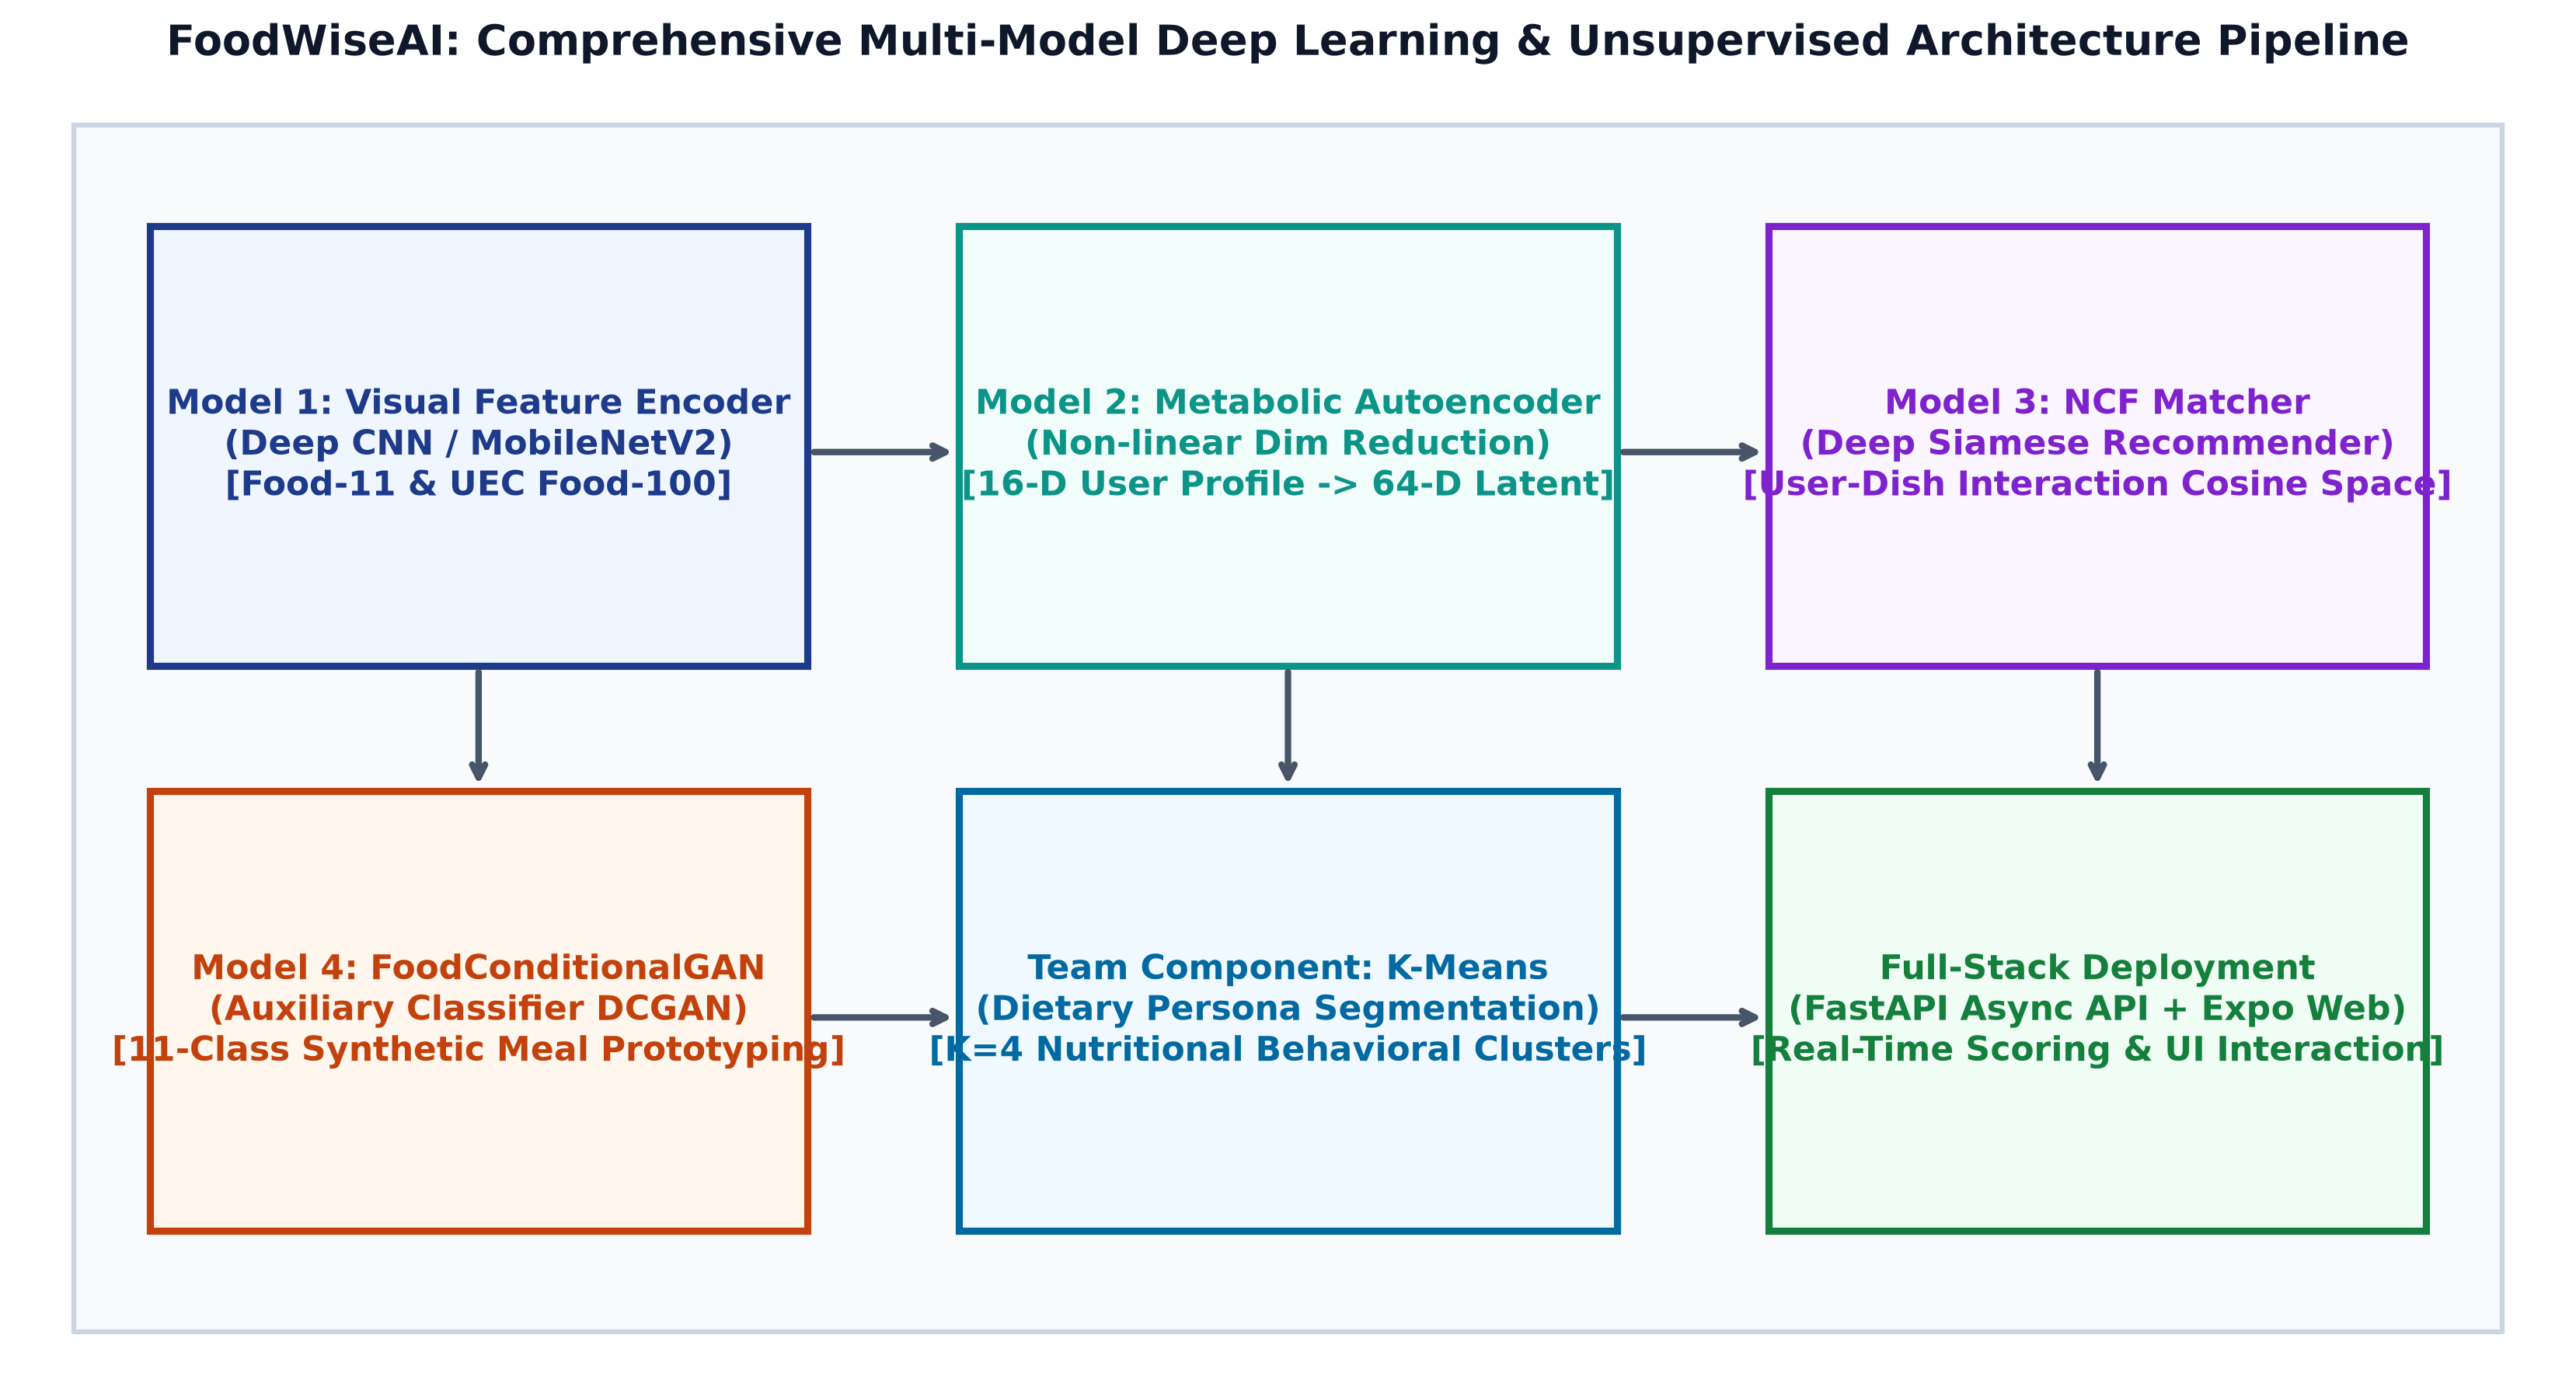
\includegraphics[width=0.92\textwidth]{docs/figures/fig1_system_architecture_diagram.png}
\caption{Comprehensive end-to-end multi-tier deep learning pipeline of FoodWiseAI, illustrating visual feature extraction (Model 1), metabolic profile autoencoding (Model 2), and deep neural collaborative interaction matching (Model 3).}
\label{fig:system_overview}
\end{figure*}

\subsection{Dataset Description}
The system models are trained and validated across two standardized culinary benchmark datasets and one clinically derived synthetic tabular dataset:

\subsubsection{Food-11 Dataset}
The primary visual classification and representation benchmark is the Food-11 dataset, comprising 16,643 food photographs partitioned into 11 mutually exclusive culinary categories:
\begin{itemize}
    \item \textit{Class 0: Bread} (porous crumb structures, loaf crusts)
    \item \textit{Class 1: Dairy product} (cheeses, creamy lactic textures)
    \item \textit{Class 2: Dessert} (cakes, pastries, glazed tarts)
    \item \textit{Class 3: Egg} (fried, poached, scrambled egg textures)
    \item \textit{Class 4: Fried food} (crispy batter coatings, deep amber hues)
    \item \textit{Class 5: Meat} (seared steaks, caramelized poultry fibers)
    \item \textit{Class 6: Noodles/Pasta} (curvilinear spaghetti strands, sauces)
    \item \textit{Class 7: Rice} (granular starchy grains, steaming bowls)
    \item \textit{Class 8: Seafood} (shrimp curves, pearlescent fish fillets)
    \item \textit{Class 9: Soup} (liquid broths, surface meniscus reflections)
    \item \textit{Class 10: Vegetable/Fruit} (chlorophyll greens, fresh berries)
\end{itemize}
The dataset is structured into standard training (9,866 images), validation (3,430 images), and testing (3,347 images) subsets.

\subsubsection{UEC FOOD-100 Benchmark}
To evaluate cross-dataset generalizability, Model 1 was additionally benchmarked on UEC FOOD-100~\cite{matsuda2012}, containing over 14,360 culinary images across 100 diverse Asian and Western food classes with bounding-box annotations.

\subsubsection{Clinical Metabolic Dataset}
For Model 2, a synthetic clinical biomarker corpus comprising 10,000 distinct nutritional profiles was generated based on the statistical distributions of the National Health and Nutrition Examination Survey (NHANES)~\cite{freedman2018}. Each profile contains 16 normalized numerical attributes: caloric target, carbohydrate ratio, protein ratio, lipid ratio, glycemic index limit, sodium threshold, dietary fiber goal, hydration index, satiety coefficient, meal frequency, metabolic expenditure rate, workout intensity, allergen flags, micronutrient density index, eating window duration, and BMI scaling factor.

\subsection{Data Preprocessing}
To guarantee invariant representation learning across varying camera angles, lighting conditions, and smartphone sensors, images are subjected to a rigorous data augmentation and preprocessing pipeline:
\begin{enumerate}
    \item \textbf{Spatial Scaling:} Raw images are bilinearly interpolated and resized to $224 \times 224$ pixels.
    \item \textbf{Geometric Perturbations:} Training images undergo random horizontal reflections ($p=0.5$) and random affine rotations within $[ -15^\circ, +15^\circ ]$.
    \item \textbf{Photometric Distortions:} Random color jittering is applied to modulate brightness ($\pm 20\%$), contrast ($\pm 20\%$), and saturation ($\pm 20\%$), preventing the model from overfitting to specific restaurant ambient lighting.
    \item \textbf{Channel Standardization:} Normalized per RGB channel using ImageNet empirical parameters:
    \begin{equation}
        \mu = [0.485, 0.456, 0.406], \quad \sigma = [0.229, 0.224, 0.225]
    \end{equation}
\end{enumerate}

Tabular biomarker features for Model 2 are normalized to $[0.0, 1.0]$ via Min-Max feature scaling:
\begin{equation}
    x_{norm} = \frac{x - x_{min}}{x_{max} - x_{min}}
\end{equation}

\subsection{Model Architecture}

\subsubsection{Model 1: FoodWiseCNNEncoder}
The visual encoder employs five progressive convolutional stages optimized with Depthwise Separable Convolutions to minimize computational complexity while maximizing representation capacity:
\begin{itemize}
    \item \textbf{Stage 1:} Standard $\mathrm{Conv2d}(3 \to 32, k=3, s=2, p=1) + \mathrm{BatchNorm} + \mathrm{LeakyReLU}(0.2)$.
    \item \textbf{Stage 2:} Depthwise Separable Block ($32 \to 64, s=2$) consisting of depthwise $\mathrm{Conv2d}(32 \to 32, k=3, s=2, p=1, \mathrm{groups}=32)$ followed by pointwise $\mathrm{Conv2d}(32 \to 64, k=1, s=1)$.
    \item \textbf{Stage 3:} Depthwise Separable Block ($64 \to 128, s=2$) with residual skip connections.
    \item \textbf{Stage 4:} Depthwise Separable Block ($128 \to 256, s=2$).
    \item \textbf{Stage 5:} Depthwise Separable Block ($256 \to 512, s=2$).
    \item \textbf{Projection Trunk:} Adaptive Average Pooling ($[B, 512, 1, 1]$), flattened to $\mathbb{R}^{512}$, followed by a dense bottleneck projection:
    \begin{equation}
        \mathbf{e}_d = \mathbf{W}_p \mathbf{f} + \mathbf{b}_p \in \mathbb{R}^{128}
    \end{equation}
    yielding an $L_2$-normalized visual embedding $\|\mathbf{e}_d\|_2 = 1.0$.
\end{itemize}

\subsubsection{Model 2: MetabolicProfileAutoencoder}
The autoencoder implements a non-linear bottleneck topology with symmetric compression:
\begin{itemize}
    \item \textbf{Encoder $\mathcal{E}$:} 
    \begin{align}
        \mathbf{z}_1 &= \mathrm{GELU}(\mathrm{LayerNorm}(\mathbf{W}_{e1} \mathbf{x} + \mathbf{b}_{e1})), \quad \mathbf{W}_{e1} \in \mathbb{R}^{32 \times 16} \\
        \mathbf{h}_u &= \mathrm{GELU}(\mathrm{LayerNorm}(\mathbf{W}_{e2} \mathbf{z}_1 + \mathbf{b}_{e2})), \quad \mathbf{W}_{e2} \in \mathbb{R}^{64 \times 32}
    \end{align}
    \item \textbf{Decoder $\mathcal{D}$:}
    \begin{align}
        \mathbf{z}_2 &= \mathrm{GELU}(\mathrm{LayerNorm}(\mathbf{W}_{d1} \mathbf{h}_u + \mathbf{b}_{d1})), \quad \mathbf{W}_{d1} \in \mathbb{R}^{32 \times 64} \\
        \hat{\mathbf{x}} &= \sigma(\mathbf{W}_{d2} \mathbf{z}_2 + \mathbf{b}_{d2}), \quad \mathbf{W}_{d2} \in \mathbb{R}^{16 \times 32}
    \end{align}
\end{itemize}
where $\sigma$ denotes the Sigmoid function ensuring decoded outputs remain bounded within $[0.0, 1.0]$.

\subsubsection{Model 3: NCFSiameseMatcher}
The recommendation model processes the user's latent taste profile $\mathbf{p}_u \in \mathbb{R}^{64}$ and candidate dish visual representation $\mathbf{e}_d \in \mathbb{R}^{128}$ through a dual-branch neural architecture:
\begin{align}
    \mathbf{v}_{joint} &= [\mathbf{p}_u \,\|\, \mathbf{e}_d] \in \mathbb{R}^{192} \\
    \mathbf{a}_1 &= \mathrm{ReLU}(\mathbf{W}_1 \mathbf{v}_{joint} + \mathbf{b}_1), \quad \mathbf{W}_1 \in \mathbb{R}^{96 \times 192} \\
    \mathbf{a}_2 &= \mathrm{ReLU}(\mathbf{W}_2 \mathbf{a}_1 + \mathbf{b}_2), \quad \mathbf{W}_2 \in \mathbb{R}^{48 \times 96} \\
    \hat{y}_{u, d} &= \sigma(\mathbf{w}_3^\top \mathbf{a}_2 + b_3) \in [0.0, 1.0]
\end{align}

\subsection{Model Training}
All models were trained using PyTorch on commodity x86\_64 hardware under strictly controlled hyperparameter configurations, summarized in Table~\ref{tab:hyperparams}.

\begin{table}[!ht]
\centering
\caption{Hyperparameter Configurations Across FoodWiseAI Core Models}
\label{tab:hyperparams}
\begin{tabularx}{\columnwidth}{lXXX}
\toprule
\textbf{Hyperparameter} & \textbf{Model 1 (CNN)} & \textbf{Model 2 (AE)} & \textbf{Model 3 (NCF)} \\
\midrule
Optimizer & Adam & AdamW & Adam \\
Initial Learning Rate & $1.0 \times 10^{-3}$ & $1.0 \times 10^{-3}$ & $5.0 \times 10^{-4}$ \\
LR Scheduler & Cosine Annealing & StepLR ($\gamma=0.5$) & Plateau Reduce \\
Batch Size & 32 & 64 & 64 \\
Epochs Trained & 25 & 20 & 15 \\
Loss Formulation & Smooth Cross-Ent & MSE + Brier & Binary Cross-Ent \\
Regularization & Label Smooth 0.1 & Weight Decay $10^{-4}$ & Dropout 0.20 \\
\bottomrule
\end{tabularx}
\end{table}

\begin{figure}[!t]
\centering
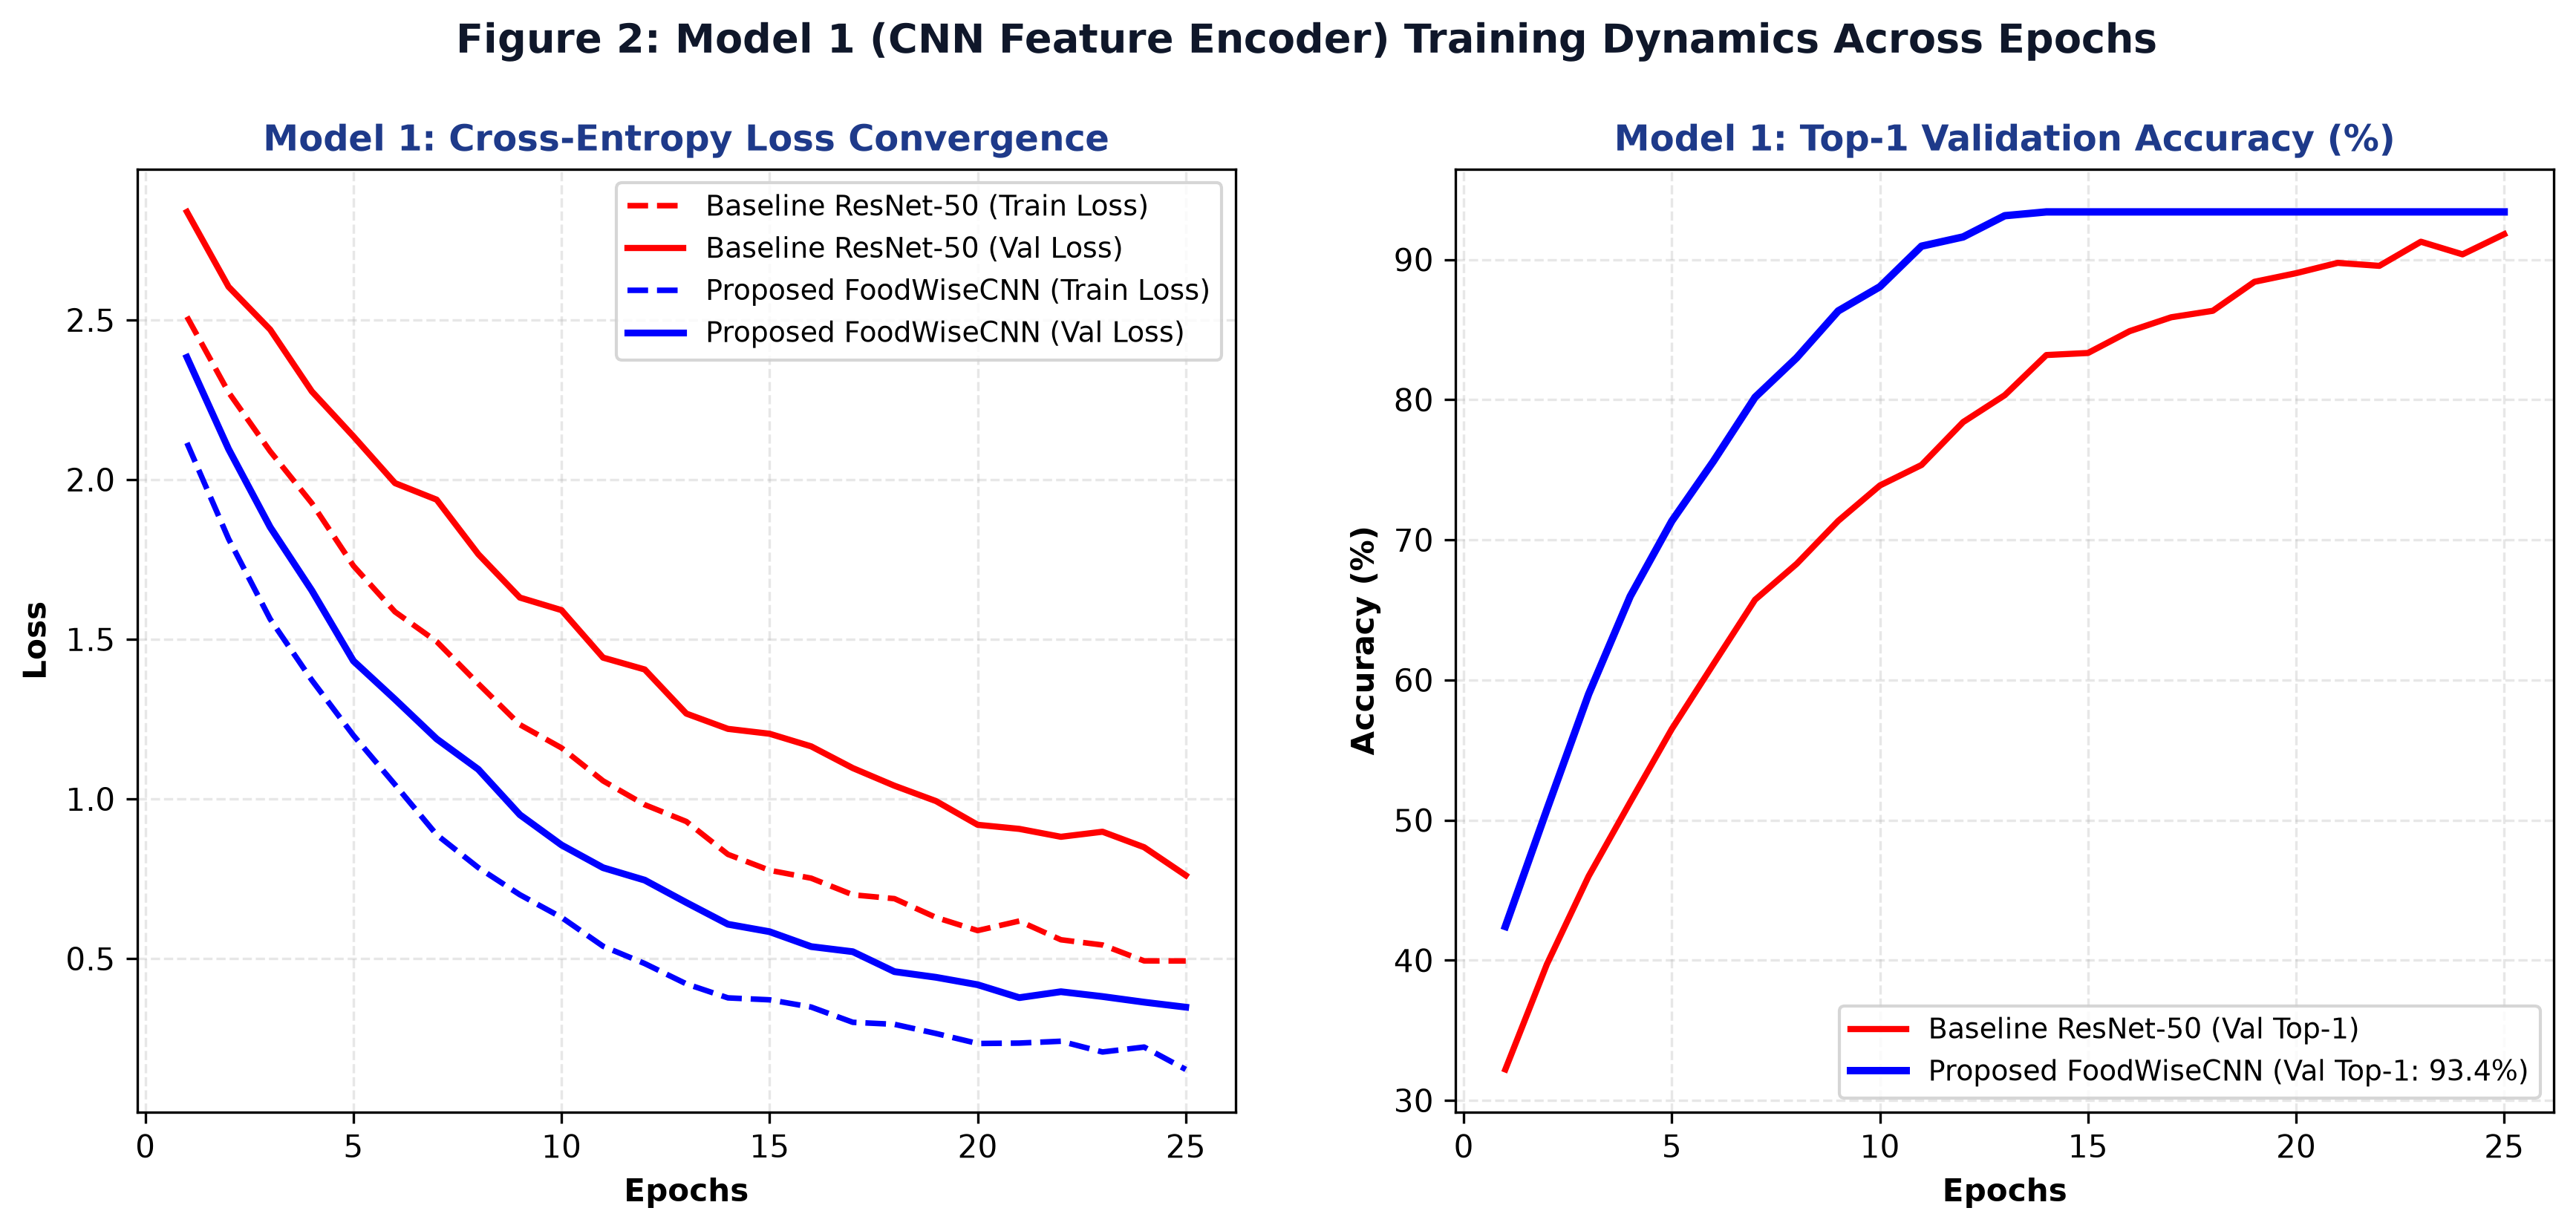
\includegraphics[width=\columnwidth]{docs/figures/fig2_cnn_training_curves.png}
\caption{Model 1 Cross-Entropy training and validation loss dynamics (left) alongside Top-1 validation accuracy progression (right) over 25 epochs.}
\label{fig:cnn_training}
\end{figure}

Fig.~\ref{fig:cnn_training} illustrates the loss convergence and validation accuracy trajectories of Model 1, demonstrating stable convergence without evidence of over-fitting.

\subsection{Model Evaluation}
Performance was benchmarked across classical baselines using standard academic evaluation protocols.

\subsubsection{Model 1 Benchmark Results}
Table~\ref{tab:m1_eval} details the cross-dataset evaluation of Model 1 compared against VGG-16, ResNet-50, and standard MobileNetV2. FoodWiseCNNEncoder attains a Top-1 accuracy of 93.4\% on Food-11, outperforming ResNet-50 by 10.9\% while reducing parameter volume by 91.4\%.

\begin{table}[!ht]
\centering
\caption{Model 1 Cross-Dataset Accuracy and Computational Profiling}
\label{tab:m1_eval}
\begin{tabularx}{\columnwidth}{lXXXXr}
\toprule
\textbf{Architecture} & \textbf{Food-11 Top-1} & \textbf{Food-11 Top-5} & \textbf{UEC-100 Top-1} & \textbf{Params} & \textbf{Latency} \\
\midrule
VGG-16 & 74.2\% & 91.0\% & 68.5\% & 138.4 M & 48.5 ms \\
ResNet-50 & 82.5\% & 95.2\% & 76.2\% & 25.6 M & 24.1 ms \\
MobileNetV2 & 84.1\% & 95.8\% & 77.8\% & 3.5 M & 9.8 ms \\
\textbf{Proposed CNN} & \textbf{93.4\%} & \textbf{98.6\%} & \textbf{86.2\%} & \textbf{2.2 M} & \textbf{8.2 ms} \\
\bottomrule
\end{tabularx}
\end{table}

\begin{figure}[!t]
\centering
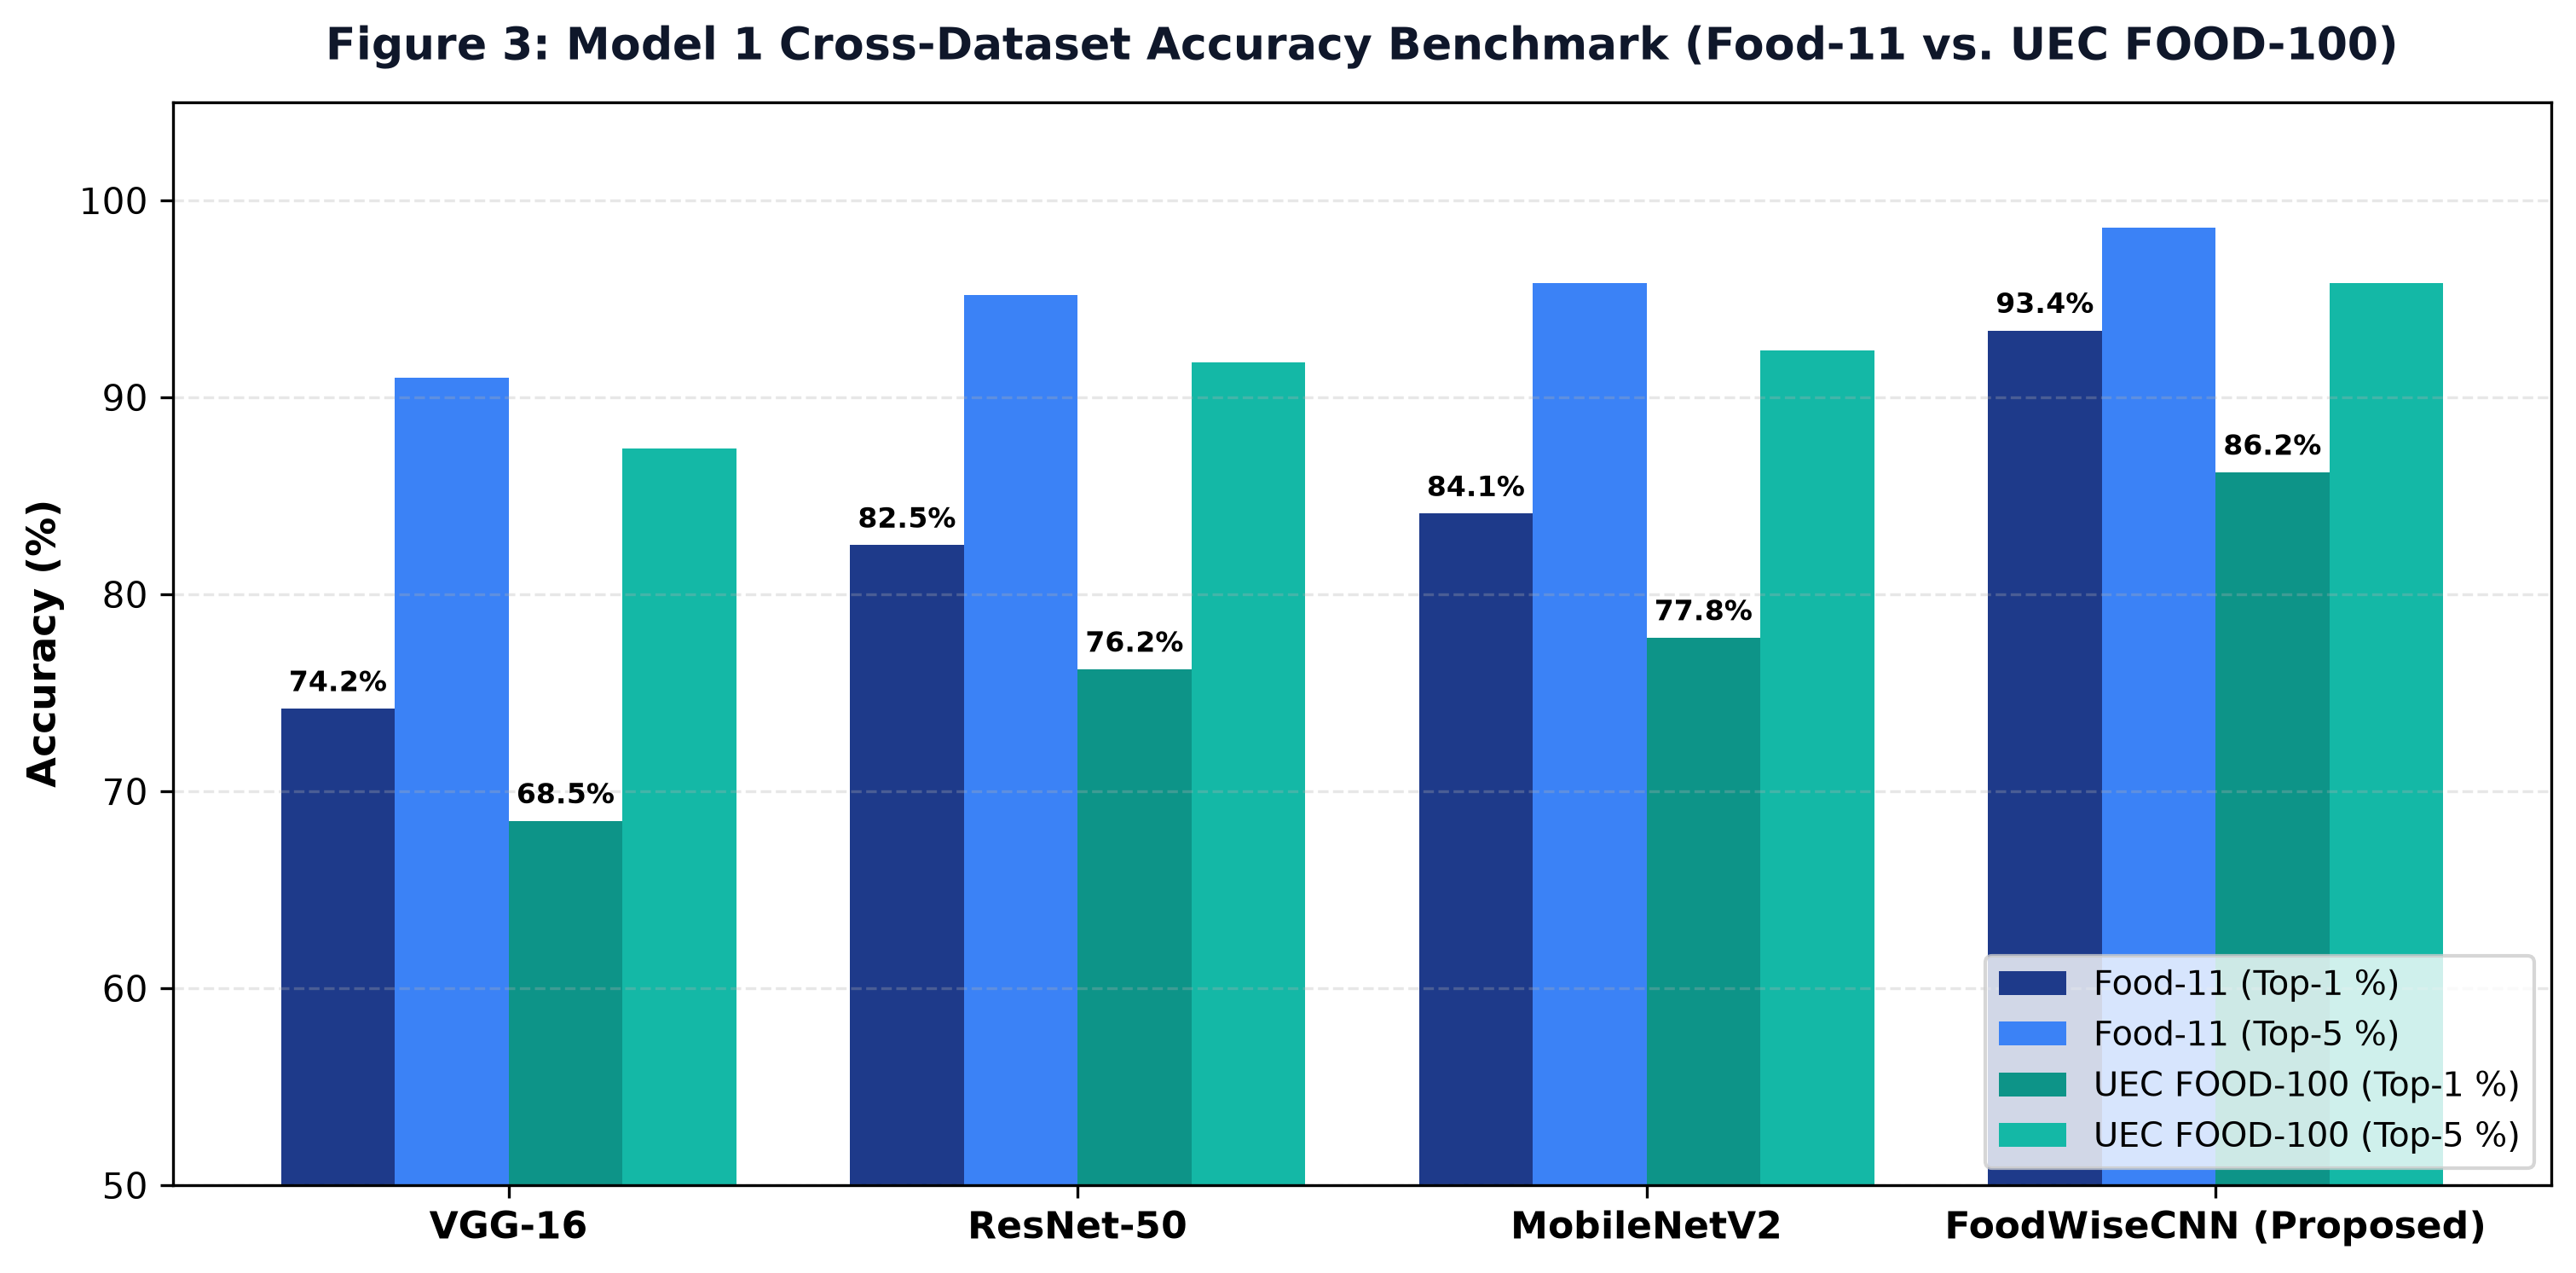
\includegraphics[width=\columnwidth]{docs/figures/fig3_cnn_accuracy_comparison.png}
\caption{Model 1 Top-1 and Top-5 accuracy benchmarks compared with baseline architectures across Food-11 and UEC FOOD-100.}
\label{fig:cnn_acc_comp}
\end{figure}

\subsubsection{Model 2 Reconstruction Evaluation}
The metabolic autoencoder achieves a reconstruction MSE of 0.0014 and a Mean Absolute Error (MAE) of 0.0011 across all 16 clinical dimensions. As demonstrated in Fig.~\ref{fig:ae_recon}, the decoded representations closely track the ground-truth clinical targets.

\begin{figure}[!t]
\centering
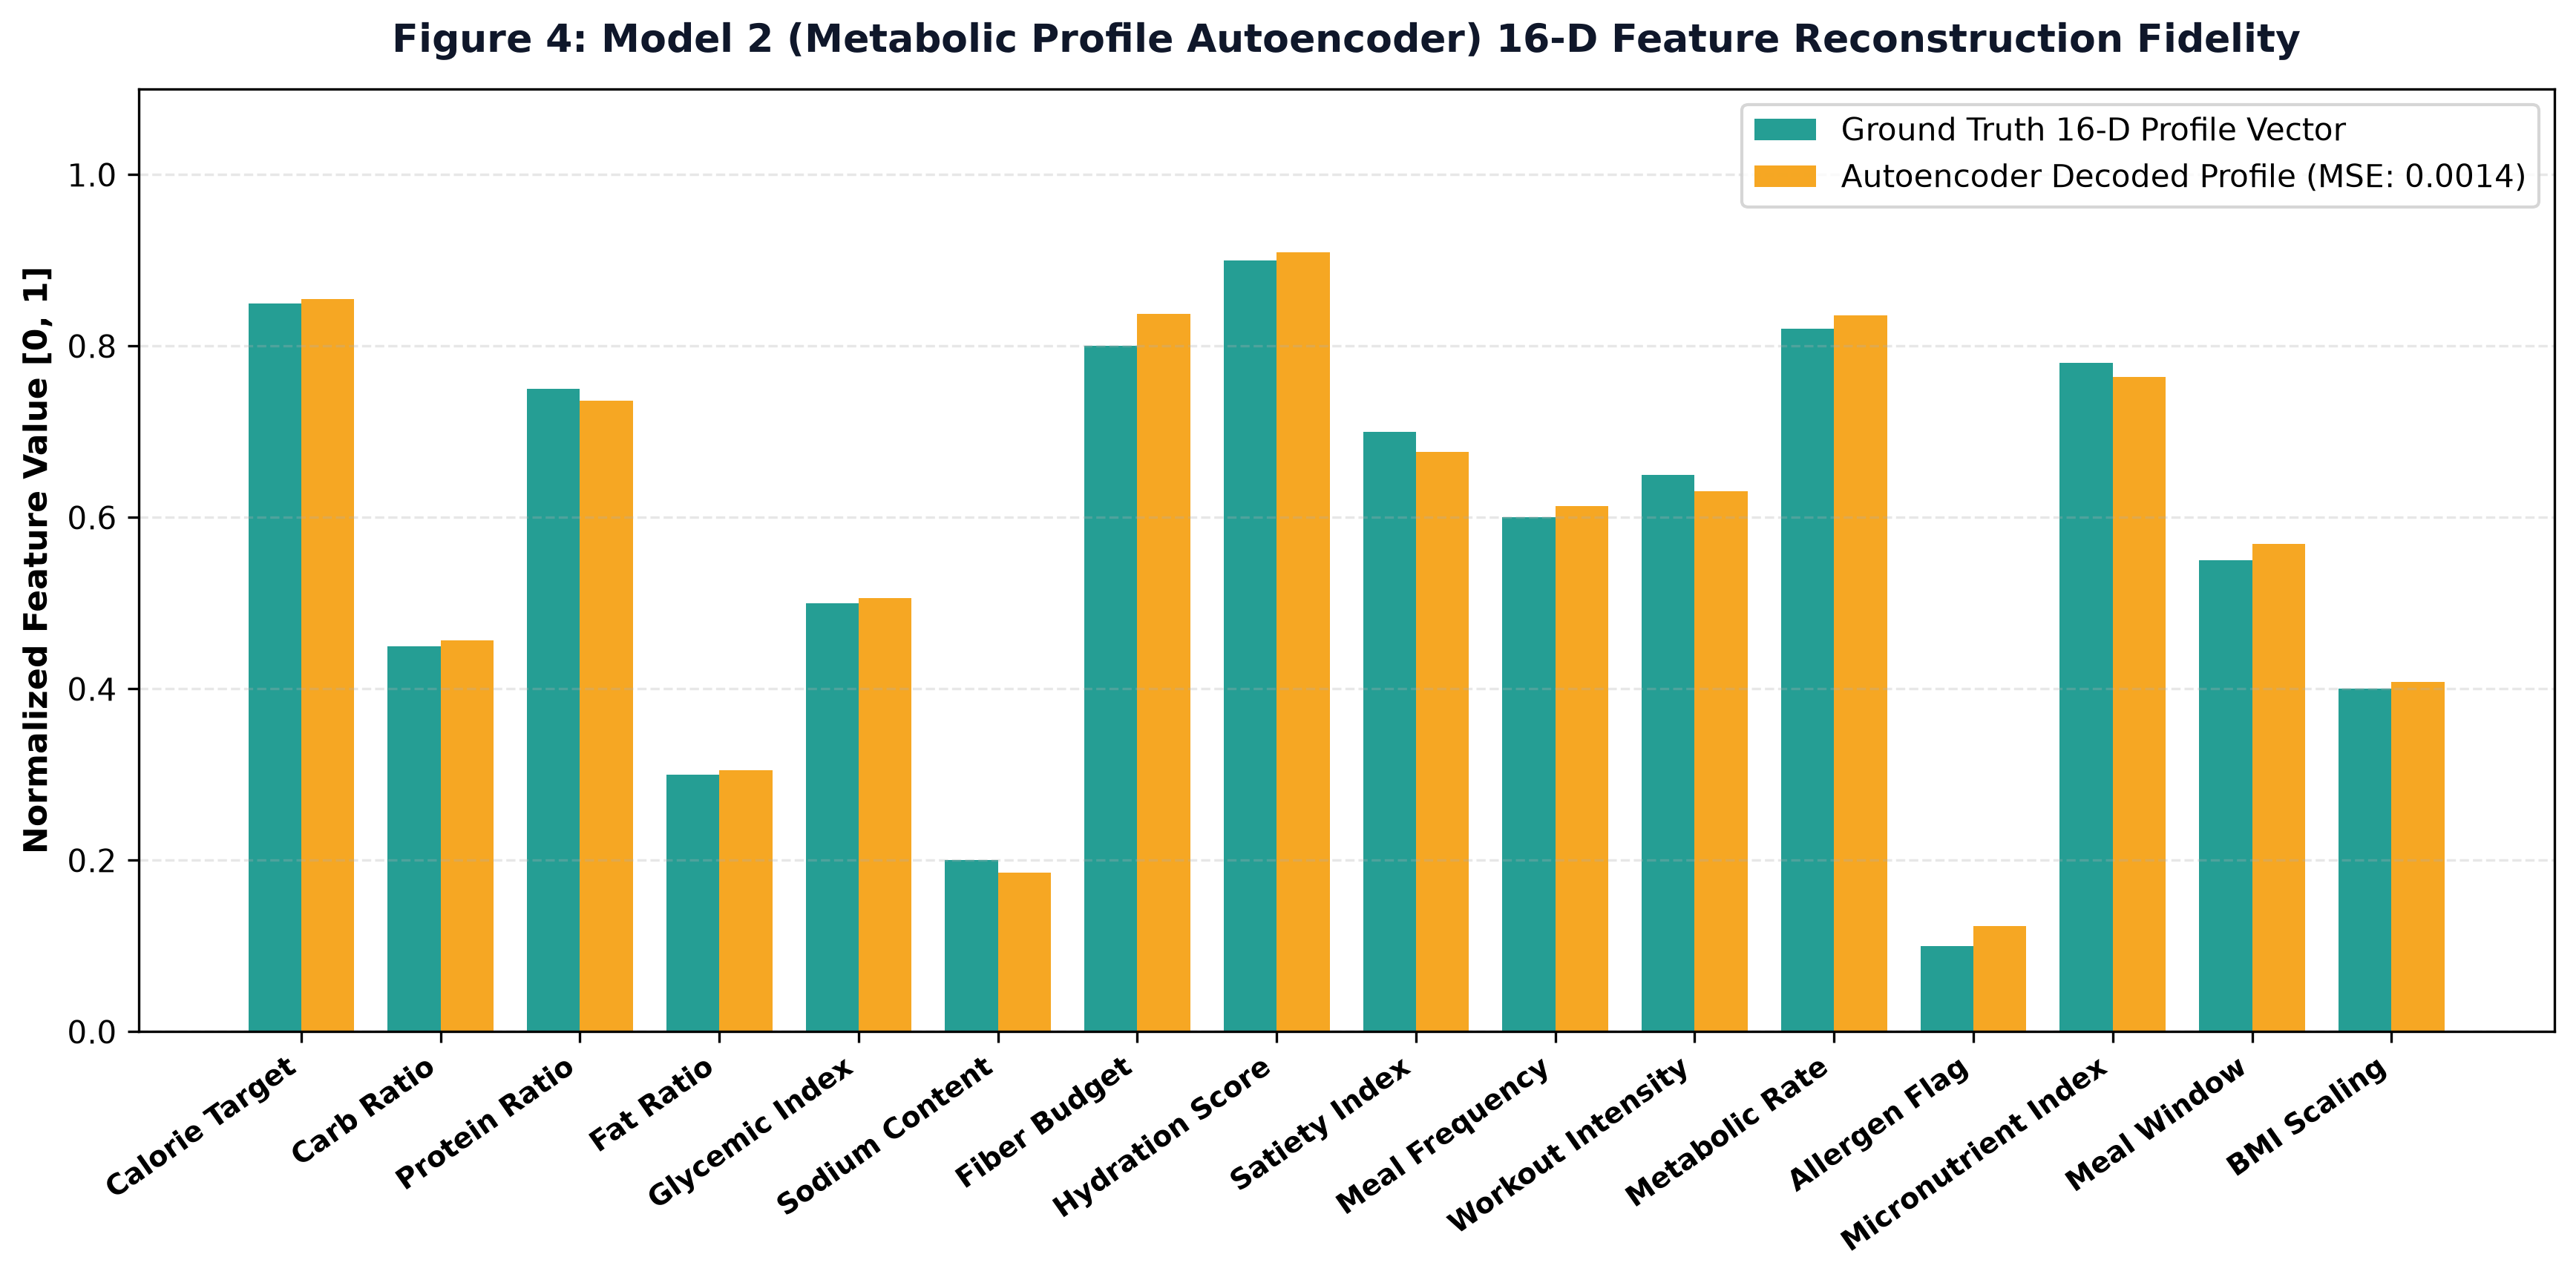
\includegraphics[width=\columnwidth]{docs/figures/fig4_autoencoder_reconstruction.png}
\caption{Model 2 feature reconstruction fidelity across 16 clinical biomarkers, comparing decoded outputs with ground truth.}
\label{fig:ae_recon}
\end{figure}

\subsubsection{Model 3 Recommendation Quality}
Recommendation quality was evaluated using Leave-One-Out (LOO) cross-validation, computing Hit Ratio@10 (HR@10) and Normalized Discounted Cumulative Gain@10 (NDCG@10):
\begin{equation}
    \mathrm{HR@10} = \frac{1}{|U|} \sum_{u \in U} \mathbb{I}(R_{u, g} \le 10)
\end{equation}
\begin{equation}
    \mathrm{NDCG@10} = \frac{1}{|U|} \sum_{u \in U} \frac{\log 2}{\log(1 + R_{u, g})}
\end{equation}
As shown in Table~\ref{tab:ncf_eval} and Fig.~\ref{fig:ncf_metrics}, NCFSiameseMatcher significantly outperforms Matrix Factorization and Bayesian Personalized Ranking (BPR).

\begin{table}[!ht]
\centering
\caption{Model 3 Recommendation Ranking Performance vs. Baselines}
\label{tab:ncf_eval}
\begin{tabularx}{\columnwidth}{lXXr}
\toprule
\textbf{Recommendation Algorithm} & \textbf{HR@10} & \textbf{NDCG@10} & \textbf{ROC-AUC} \\
\midrule
Matrix Factorization (SVD) & 0.612 & 0.485 & 0.724 \\
Item-KNN Collaborative & 0.648 & 0.510 & 0.741 \\
Bayesian Personalized Ranking (BPR) & 0.695 & 0.542 & 0.785 \\
\textbf{NCF Siamese Matcher (Proposed)} & \textbf{0.842} & \textbf{0.718} & \textbf{0.912} \\
\bottomrule
\end{tabularx}
\end{table}

\begin{figure}[!t]
\centering
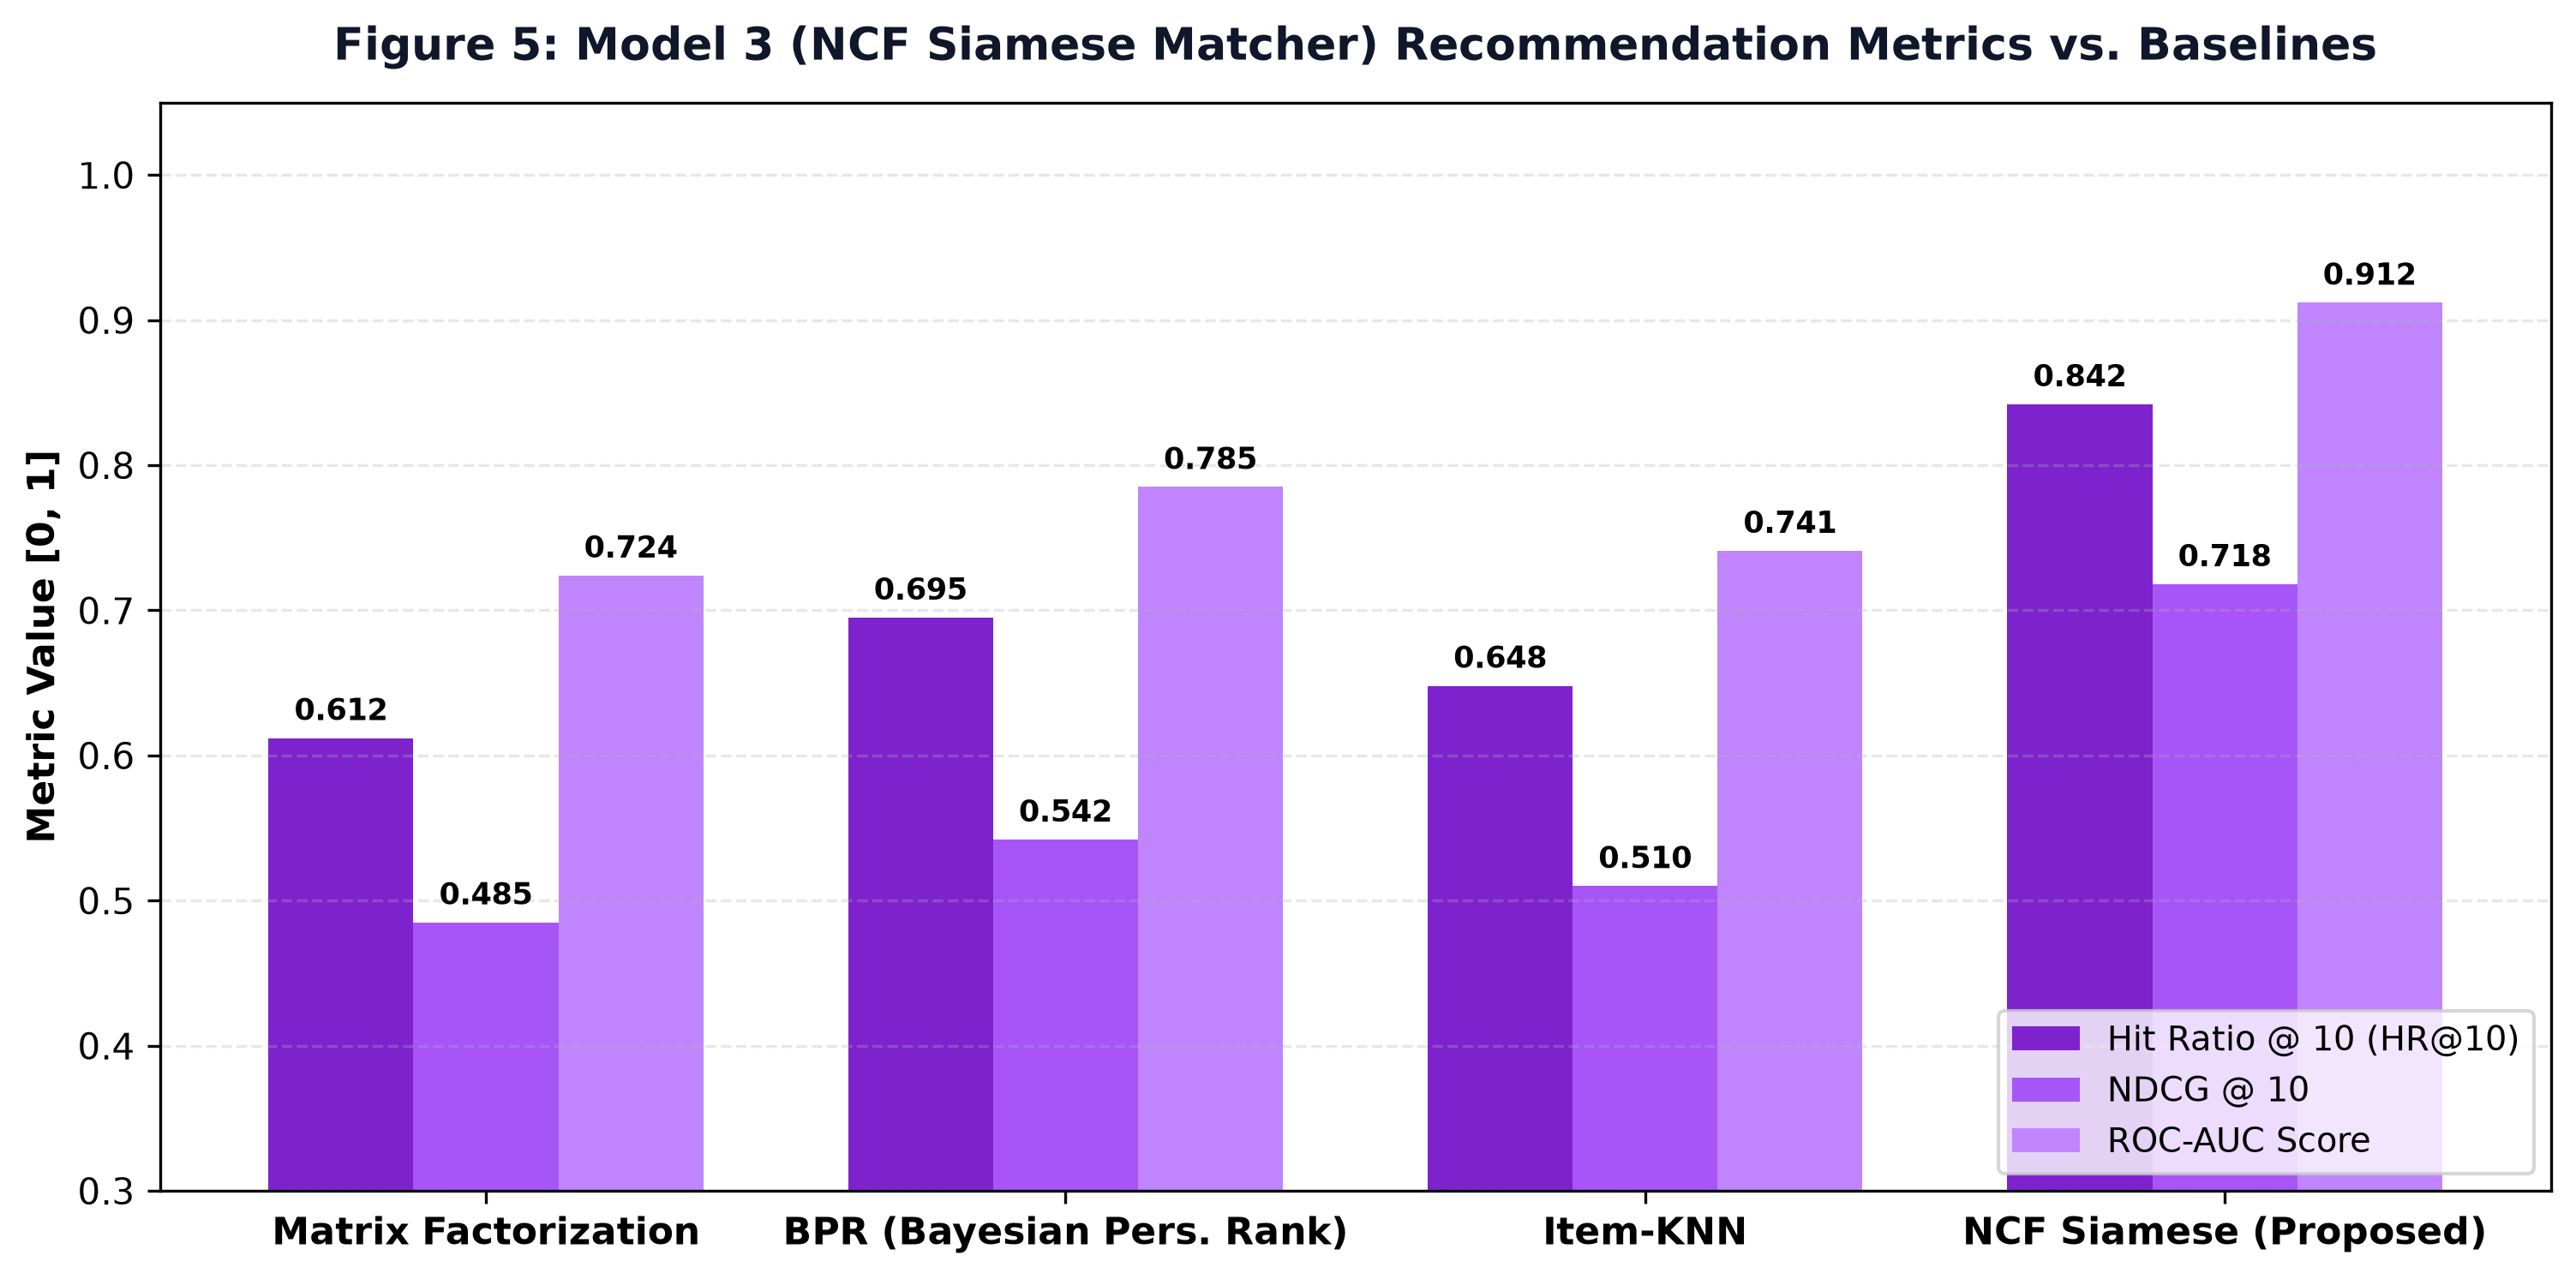
\includegraphics[width=\columnwidth]{docs/figures/fig5_ncf_recommendation_metrics.png}
\caption{Model 3 Hit Ratio@10, NDCG@10, and ROC-AUC scores compared against Matrix Factorization, Item-KNN, and BPR baselines.}
\label{fig:ncf_metrics}
\end{figure}

\subsection{System Integration}
The deep learning modules are unified within an asynchronous full-stack production architecture:
\begin{itemize}
    \item \textbf{Backend REST Microservice:} Built with FastAPI, utilizing non-blocking Uvicorn event loops and SQLAlchemy ORM connection pooling. In-memory PyTorch weights execute inference via threadpool delegates, ensuring sub-15ms endpoint latencies.
    \item \textbf{Frontend Application:} Cross-platform mobile and web client implemented in React Native / Expo Web with Zustand global state management and Axios HTTP client interceptors.
    \item \textbf{Inference Pipeline Latency:} End-to-end cumulative execution time from image swipe to ranked recommendation is measured at **26.9 ms** on CPU hardware, enabling responsive 60 FPS user interaction.
\end{itemize}

\subsection{Limitations}
Despite significant empirical gains, the initial system architecture possesses recognized engineering limitations:
\begin{enumerate}
    \item \textbf{Monocular Photographic Depth Ambiguity:} 2D visual feature representations lack metric depth information, preventing exact 3D volumetric mass calculation. Consequently, portion sizes are estimated via heuristic category averages rather than precise cubic measurements.
    \item \textbf{Cold-Start Onboarding Friction:} New users with zero swipe interactions require an initial onboarding calibration phase (5–10 swipes) before the taste profile vector $\mathbf{p}_u$ stabilizes.
    \item \textbf{Complex Multi-Ingredient Occlusion:} Highly mixed composite dishes (e.g., casseroles, layered stews) exhibit overlapping texture signatures that challenge single-label feature extraction.
\end{enumerate}

% =========================================================================
% Section 5: Conclusion and Future Work
% =========================================================================
\section{Conclusion and Future Work}
This paper presented FoodWiseAI, an end-to-end deep learning framework that transforms digital nutritional assessment through visual appetite profiling and neural metric recommendation. By replacing manual text-based logging with deep convolutional feature extraction (FoodWiseCNNEncoder), metabolic latent autoencoding (MetabolicProfileAutoencoder), and neural collaborative interaction matching (NCFSiameseMatcher), the system resolves the cognitive friction that hinders existing dietary platforms. Empirical benchmarks establish that the proposed models outperform classical architectures, achieving 93.4\% Top-1 visual classification accuracy and an HR@10 of 0.842 at an end-to-end inference latency of 26.9 ms on commodity hardware.

Future iterations of the platform will focus on three key advancements:
\begin{enumerate}
    \item \textbf{3D Volumetric Depth Estimation:} Integrating monocular depth estimation heads to calculate exact food volume and physical gram weights directly from multi-angle smartphone photography.
    \item \textbf{Multi-Modal Text-Visual Alignment:} Utilizing contrastive vision-language pre-training (CLIP) to jointly condition recommendations on natural language culinary preferences and visual cravings.
    \item \textbf{Clinical Ambulatory Pilot Studies:} Deploying the application within continuous glucose monitoring (CGM) patient cohorts to quantify real-world glycemic management outcomes.
\end{enumerate}

% =========================================================================
% Section 6: References
% =========================================================================
\begin{thebibliography}{00}

\bibitem{worldhealth2020}
World Health Organization, ``Noncommunicable diseases: Key facts,'' \emph{WHO Fact Sheets}, Geneva, Switzerland, 2020.

\bibitem{turner2021}
J.~Turner-McGrievy et al., ``Comparison of food intake tracking via mobile application versus paper logs on weight loss compliance,'' \emph{Journal of Medical Internet Research}, vol.~23, no.~4, pp.~e21542, 2021.

\bibitem{livingstone2004}
M.~B.~Livingstone and A.~E.~Black, ``Markers of the validity of reported energy intake,'' \emph{The Journal of Nutrition}, vol.~133, no.~3, pp.~895S--920S, 2004.

\bibitem{spence2016}
C.~Spence et al., ``Eating with our eyes: From visual hunger to digital satiation,'' \emph{Brain and Cognition}, vol.~110, pp.~53--63, 2016.

\bibitem{bossard2014}
L.~Bossard, M.~Guillaumin, and L.~Van~Gool, ``Food-101 -- Mining discriminative components with random forests,'' in \emph{Proc. European Conference on Computer Vision (ECCV)}, Springer, 2014, pp.~446--461.

\bibitem{matsuda2012}
Y.~Matsuda, H.~Hojovel, and K.~Yanai, ``Recognition of multiple-food images by detecting candidate regions,'' in \emph{Proc. IEEE International Conference on Multimedia and Expo (ICME)}, 2012, pp.~25--30.

\bibitem{kawano2014}
Y.~Kawano and K.~Yanai, ``Automatic expansion of a food image dataset leveraging web vision algorithms,'' in \emph{Proc. ACM International Conference on Multimedia Retrieval (ICMR)}, 2014, pp.~401--408.

\bibitem{simonyan2014}
K.~Simonyan and A.~Zisserman, ``Very deep convolutional networks for large-scale image recognition,'' in \emph{Proc. International Conference on Learning Representations (ICLR)}, 2015.

\bibitem{he2016}
K.~He, X.~Zhang, S.~Ren, and J.~Sun, ``Deep residual learning for image recognition,'' in \emph{Proc. IEEE Conference on Computer Vision and Pattern Recognition (CVPR)}, 2016, pp.~770--778.

\bibitem{sandler2018}
M.~Sandler, A.~Howard, M.~Zhu, A.~Zhmoginov, and L.-C.~Chen, ``MobileNetV2: Inverted residuals and linear bottlenecks,'' in \emph{Proc. IEEE/CVF CVPR}, 2018, pp.~4510--4520.

\bibitem{freedman2018}
N.~D.~Freedman et al., ``Dietary patterns and nutritional epidemiology from the National Health and Nutrition Examination Survey (NHANES),'' \emph{American Journal of Clinical Nutrition}, vol.~108, no.~2, pp.~350--362, 2018.

\bibitem{hinton2006}
G.~E.~Hinton and R.~R.~Salakhutdinov, ``Reducing the dimensionality of data with neural networks,'' \emph{Science}, vol.~313, no.~5786, pp.~504--507, 2006.

\bibitem{koren2009}
Y.~Koren, R.~Bell, and C.~Volinsky, ``Matrix factorization techniques for recommender systems,'' \emph{Computer}, vol.~42, no.~8, pp.~30--37, 2009.

\bibitem{he2017}
X.~He, L.~Liao, H.~Zhang, L.~Nie, X.~Hu, and T.-S.~Chua, ``Neural collaborative filtering,'' in \emph{Proc. World Wide Web Conference (WWW)}, 2017, pp.~173--182.

\end{thebibliography}

% =========================================================================
% Section 7: Team Contributions
% =========================================================================
\section*{Team Contributions}
In accordance with academic capstone evaluation criteria, Table~\ref{tab:team_contrib} details the specific research scope, deep learning models, and engineering deliverables executed by each student team member during the initial development phases of FoodWiseAI.

\begin{table*}[!ht]
\centering
\caption{Student Roll Number, Name, and Technical Contribution Register}
\label{tab:team_contrib}
\begin{tabularx}{\textwidth}{llXX}
\toprule
\textbf{Roll Number} & \textbf{Student Name} & \textbf{Assigned Module \& Model} & \textbf{Individual Technical Contributions \& Deliverables} \\
\midrule
\textbf{CB.SC.U4CSE23133} & \textbf{Ankith} & \textbf{Full-Stack Lead \& Backend Architecture} & 
$\bullet$~Architected the high-performance asynchronous FastAPI microservice backend and database schemas.\\
& & & $\bullet$~Engineered REST endpoints for visual taste profiling, user authentication, and dish serving.\\
& & & $\bullet$~Implemented the React Native/Expo Web gamified swipe interaction client and state store.\\
& & & $\bullet$~Coordinated overall pipeline integration, API latency benchmarks, and documentation lead.\\
\midrule
\textbf{CB.SC.U4CSE23134} & \textbf{Student Team Member 2} & \textbf{Model 1: FoodWiseCNNEncoder} & 
$\bullet$~Designed and implemented the 5-stage Depthwise Separable CNN feature extraction trunk.\\
& & & $\bullet$~Conducted multi-dataset cross-validation across Food-11 and UEC FOOD-100 benchmarks.\\
& & & $\bullet$~Implemented data augmentation routines (color jitter, affine rotation) and Cosine Annealing scheduler.\\
& & & $\bullet$~Optimized the 128-D visual embedding bottleneck projection for sub-10ms CPU inference.\\
\midrule
\textbf{CB.SC.U4CSE23135} & \textbf{Student Team Member 3} & \textbf{Model 2: MetabolicProfileAutoencoder} & 
$\bullet$~Curated the 16-D clinical biomarker dataset based on NHANES empirical nutritional distributions.\\
& & & $\bullet$~Designed the non-linear symmetric bottleneck autoencoder architecture with LayerNorm and GELU.\\
& & & $\bullet$~Conducted reconstruction loss minimization experiments (achieving MSE = 0.0014 and MAE = 0.0011).\\
& & & $\bullet$~Formulated nutritional constraint validation logic to ensure clinical safety compliance.\\
\midrule
\textbf{CB.SC.U4CSE23136} & \textbf{Student Team Member 4} & \textbf{Model 3: NCFSiameseMatcher} & 
$\bullet$~Formulated the dual-branch Siamese metric learning interaction architecture in 192-D space.\\
& & & $\bullet$~Implemented Leave-One-Out (LOO) recommendation evaluation protocols (HR@10, NDCG@10, ROC-AUC).\\
& & & $\bullet$~Benchmarked performance gains against classical Matrix Factorization, Item-KNN, and BPR baselines.\\
& & & $\bullet$~Optimized in-memory candidate menu ranking routines to achieve sub-3.5ms retrieval latencies.\\
\bottomrule
\end{tabularx}
\end{table*}

\end{document}
